\documentclass[handout]{beamer} % Use the beamer class for presentations, 'handout' option to suppress \pause

\input{Lecture-Slides/preamble.txt}

% Title and Author Info
\title{Introduction to Statistical Methods in Political Science}
\subtitle{Lecture 3: Summarizing Data II - Graphs}
\author{Ignacio Urbina}
\date{}

%%%%%%%%%%%%%%%%%%%%%%%%%%%%%%%%%%%%%%%%%%%%%%%%%%%%%%%%%%%%%%%%%%%%%%%%%%%%%%
%%% DATA

\begin{filecontents*}{data.csv}
22, 26, 30, 17, 45
10, 15, 13, 12, 17
12, 30, 6,  57, 10
33, 38, 36, 25, 24
\end{filecontents*}

\begin{filecontents*}{data2.csv}
22, 26, 30, 17, 45, 10, 15, 13, 12, 17, 12, 30, 6,  57, 10,
33, 38, 36, 25, 24
\end{filecontents*}


%%%%%%%%%%%%%%%%%%%%%%%%%%%%%%%%%%%%%%%%%%%%%%%%%%%%%%%%%%%%%%%%%%%%%%%%%%%%%
%%% BEGIN DOC

\begin{document}

% Title slide
\begin{frame}
    \titlepage
\end{frame}

%%%%%%%%%%%%%%%%%%%%%%%%%%%%%%%%%%%%%%%%%%%%%%%%%%%%%%%%%%%%%%%%%%%%%%%%%%%
\section{Shape of a Distribution}
\transitionslide{Shape of a Distribution}

% Slide 1: Overview of Distribution Shapes
\begin{frame}{Distribution of a Variable}

A variable's distribution is a description (function) that shows its possible values and the frequency with which they occur.

By examining a variable's distribution, we learn how likely is a given value relative to others.

\end{frame}

\begin{frame}{Dot Plot Example with Discrete Numerical Data}

\begin{columns}[T,onlytextwidth]
    % Left column (larger)
    \begin{column}{0.45\textwidth}
        \textbf{Sample:}\\[6pt]
        \fbox{%
        \parbox{0.9\textwidth}{%
        \centering
        \{\,9, 10, 4, 3, 8, 9, 3, 9, 5, 2, 4, 4, 8, 9, 9, 7\}
        }}\\[10pt]
        \pause

        \textbf{Frequency Table:}
        { \scriptsize
        \begin{center}
            \begin{tabular}{lc}
                \toprule
                Value & Frequency \\
                \midrule
                2 & 1 \\
                3 & 2 \\
                4 & 3 \\
                5 & 1 \\
                6 & 0 \\
                7 & 1 \\
                8 & 2 \\
                9 & 5 \\
                10 & 1 \\
                \bottomrule
            \end{tabular}
        \end{center}
        }
        \pause
    \end{column}

    % Right column (larger) with dot plot
    \begin{column}{0.55\textwidth}
    \vspace{4em}
    \centering
    { \centering \hspace{3em} \scriptsize \textbf{Distribution of the Data} }
    \begin{tikzpicture}
        \begin{axis}[
            axis lines=left,
            xmin=1, xmax=11,
            ymin=0,  ymax=6.5,
            xtick={2,3,4,5,6,7,8,9,10},
            ytick={1,2,3,4,5},
            xlabel={\scriptsize Value},
            ylabel={\scriptsize Frequency},
            width=1.0\textwidth,
            height=0.8\textwidth,
            domain=2:10,
            clip=false,
            every axis plot/.append style={mark=*, mark options={fill=blue}, only marks}
        ]

        % Frequencies for each observed value
        %   value/frequency
        \foreach \x/\f in {
           2/1,  % One dot at x=2
           3/2,  % Two dots at x=3
           4/3,  % Three dots at x=4
           5/1,
           7/1,
           8/2,
           9/5,  % Five dots at x=9
           10/1
        }{
           % Plot each dot above the previous one
           \foreach \n in {1,...,\f}{
              \addplot coordinates {(\x, \n)};
           }
        }

        \end{axis}
    \end{tikzpicture}
    \end{column}
\end{columns}

\end{frame}



\begin{frame}{Identifying Distribution Shapes}
    \textbf{Key Distribution Shapes:}
    \begin{itemize}
        \item \textbf{Symmetric:} Equal spread on both sides.
        \item \textbf{Right Skewed:} Tail on the right (positive skewness).
        \item \textbf{Left Skewed:} Tail on the left (negative skewness).
    \end{itemize}
    \vspace{0.5cm}
    \textbf{Key Modalities:}
    \begin{itemize}
        \item \textbf{Unimodal:} Single peak.
        \item \textbf{Bimodal:} Two distinct peaks.
        \item \textbf{Multimodal:} More than two peaks.
        \item \textbf{Uniform:} Flat, no peaks.
    \end{itemize}
\end{frame}

% Slide 2: Symmetry and Skewness
\begin{frame}{Symmetry and Skewness}
    \textbf{Symmetric Distributions:}
    \begin{itemize}
        \item The distribution looks the same on both sides of the mean.
    \end{itemize}

    \vspace{0.3cm}
    \textbf{Skewed Distributions:}
    \begin{itemize}
        \item \textbf{Right skewed:} Long tail on the right.
        \item \textbf{Left skewed:} Long tail on the left.
    \end{itemize}

    \vspace{0.3cm}
    The direction of skewness indicates where most of the data points lie relative to the tail.
\end{frame}

% Slide 3: Skewness and Relationship Between Mean & Median
\begin{frame}{Skewness and the Mean-Median Relationship}
    \begin{itemize}
        \item In a \textbf{right-skewed distribution}, the mean is typically greater than the median due to the influence of the long tail.
        \item In a \textbf{left-skewed distribution}, the mean is typically less than the median for similar reasons.
        \item In a \textbf{symmetric distribution}, the mean and median are roughly equal.
    \end{itemize}

    \vspace{0.5cm}
    \textbf{Summary:}
    \begin{itemize}
        \item The relative position of the mean and median can indicate the skewness of a distribution.
    \end{itemize}
\end{frame}

% Slide 4: Unimodal, Bimodal, Multimodal, and Uniform Distributions
\begin{frame}{Unimodal, Bimodal, Multimodal, and Uniform Distributions}
    \begin{itemize}
        \item \textbf{Unimodal:} A distribution with one clear peak or mode.
        \item \textbf{Bimodal:} A distribution with two distinct peaks.
        \item \textbf{Multimodal:} More than two peaks, indicating multiple clusters or groups.
        \item \textbf{Uniform:} No peaks; all values have roughly the same frequency.
    \end{itemize}
    \vspace{0.5cm}
    These characteristics help describe the overall shape of the data and can indicate the presence of subpopulations.
\end{frame}

% Slide 5: Example of Skewness Using t-Distribution (Right-Skewed)
\begin{frame}{Right-Skewed Distribution Example}
    \textbf{Right-Skewed Distribution:}
    \begin{itemize}
        \item The tail extends to the right, meaning more data is concentrated on the left.
    \end{itemize}

    \begin{center}
        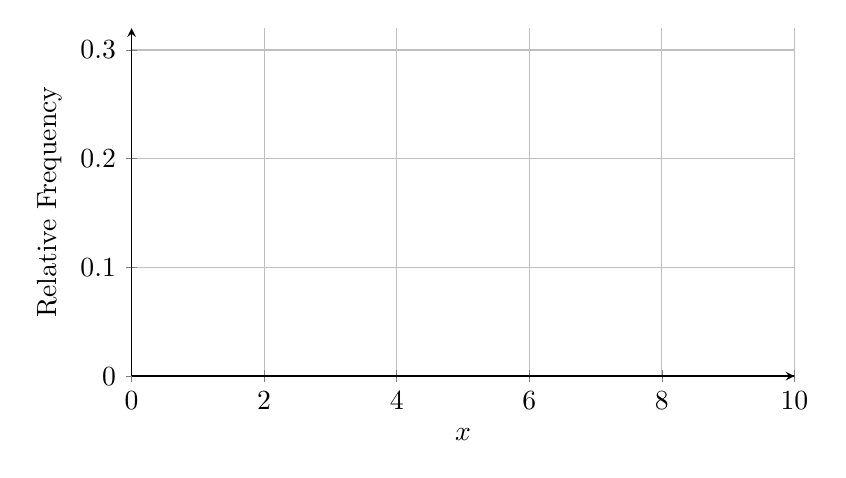
\begin{tikzpicture}
            \begin{axis}[
                domain=0:10,
                samples=100,
                xlabel=$x$,
                ylabel={Relative Frequency},
                height=6cm,
                width=10cm,
                grid=major,
                axis x line=bottom,
                axis y line=left,
                ymax=0.32
                ]
                \addplot[smooth, thick] {0};
            \end{axis}
        \end{tikzpicture}
    \end{center}
\end{frame}


% Slide 6: Left-Skewed Distribution Example
\begin{frame}{Left-Skewed Distribution Example}
    \textbf{Left-Skewed Distribution:}
    \begin{itemize}
        \item The tail extends to the left, meaning more data is concentrated on the right.
    \end{itemize}

    \begin{center}
        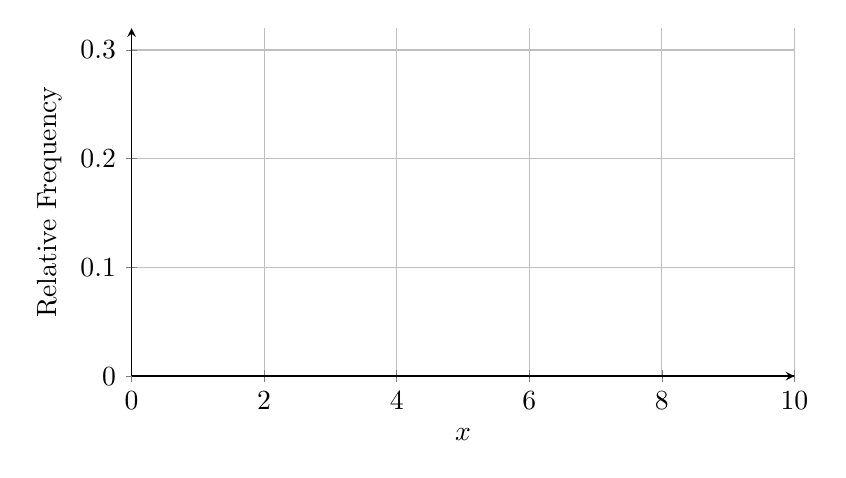
\begin{tikzpicture}
            \begin{axis}[
                domain=0:10,
                samples=100,
                xlabel=$x$,
                ylabel={Relative Frequency},
                height=6cm,
                width=10cm,
                grid=major,
                axis x line=bottom,
                axis y line=left,
                ymax=0.32
                ]
                \addplot[smooth, thick] {0};
            \end{axis}
        \end{tikzpicture}
    \end{center}
\end{frame}

% Slide 7: Symmetric Distribution Example
\begin{frame}{Symmetric Distribution Example}
    \textbf{Symmetric Distribution:}
    \begin{itemize}
        \item A symmetric distribution has equal spread on both sides of the mean.
    \end{itemize}

    \begin{center}
        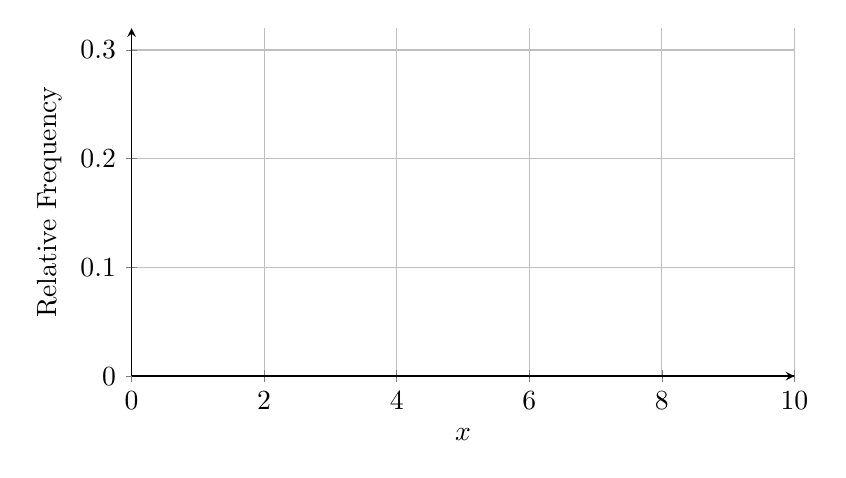
\begin{tikzpicture}
            \begin{axis}[
                domain=0:10,
                samples=100,
                xlabel=$x$,
                ylabel={Relative Frequency},
                height=6cm,
                width=10cm,
                grid=major,
                axis x line=bottom,
                axis y line=left,
                ymax=0.32
                ]
                \addplot[smooth, thick] {0};
            \end{axis}
        \end{tikzpicture}
    \end{center}
\end{frame}

\begin{frame}{Left-Skewed Distribution}
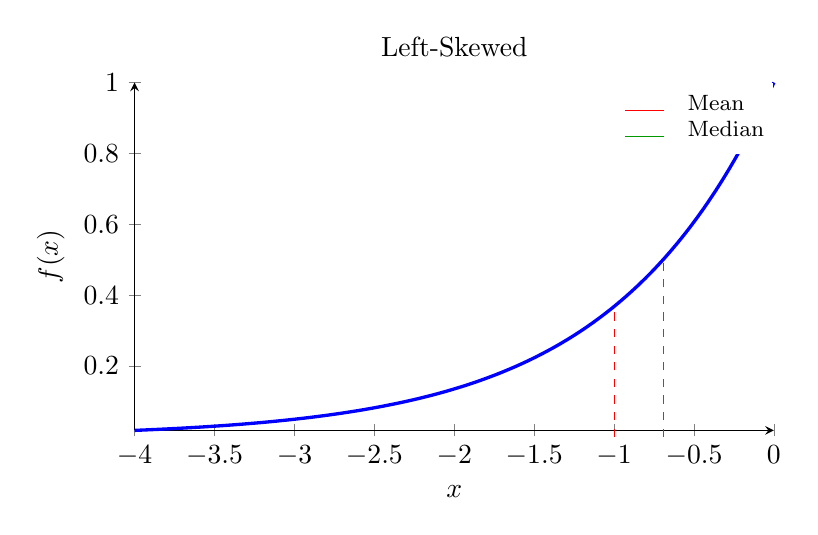
\begin{tikzpicture}
  \begin{axis}[
      domain=-4:0,
      samples=100,
      xlabel={$x$},
      ylabel={$f(x)$},
      axis lines=left,
      width=0.8\textwidth,
      height=6cm,
      title={Left-Skewed},
      clip=false
    ]
    % Plot a reflected exponential (left-skewed)
    \addplot[very thick, blue] {exp(x)};
    % Mark the mean and median
    \draw[dashed, red]   (axis cs:-1,0) -- (axis cs:-1,{exp(-1)});
    \draw[dashed, green!60!black] (axis cs:-0.693,0) -- (axis cs:-0.693,{exp(-0.693)});
    % Legend indicating the meaning of the colored lines
    \node[anchor=north east, fill=white, font=\footnotesize] at (axis description cs:1,1) {
      \begin{tabular}{@{}l@{\quad}l@{}}
      \textcolor{red}{\rule[0mm]{0.5cm}{0.1mm}} & Mean \\
      \textcolor{green!60!black}{\rule[0mm]{0.5cm}{0.1mm}} & Median \\
      \end{tabular}
    };
  \end{axis}
\end{tikzpicture}
\end{frame}


\begin{frame}{Right-Skewed Distribution}
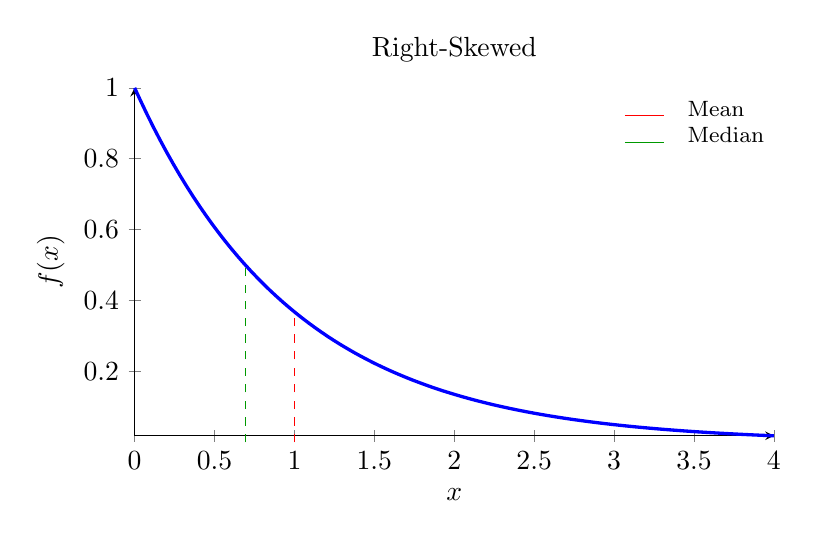
\begin{tikzpicture}
  \begin{axis}[
      domain=0:4,
      samples=100,
      xlabel={$x$},
      ylabel={$f(x)$},
      axis lines=left,
      width=0.8\textwidth,
      height=6cm,
      title={Right-Skewed},
      clip=false
    ]
    % Plot an exponential (right-skewed)
    \addplot[very thick, blue] {exp(-x)};
    % Mark the median and mean
    \draw[dashed, green!60!black] (axis cs:0.693,0) -- (axis cs:0.693,{exp(-0.693)});
    \draw[dashed, red]   (axis cs:1,0) -- (axis cs:1,{exp(-1)});
    % Legend indicating the meaning of the colored lines
    \node[anchor=north east, fill=white, font=\footnotesize] at (axis description cs:1,1) {
      \begin{tabular}{@{}l@{\quad}l@{}}
      \textcolor{red}{\rule[0mm]{0.5cm}{0.1mm}} & Mean \\
      \textcolor{green!60!black}{\rule[0mm]{0.5cm}{0.1mm}} & Median \\
      \end{tabular}
    };
  \end{axis}
\end{tikzpicture}
\end{frame}


\begin{frame}{Symmetric Distribution}


\begin{columns}[T,onlytextwidth]
    % Left column (larger)
    \begin{column}{0.75\textwidth}
        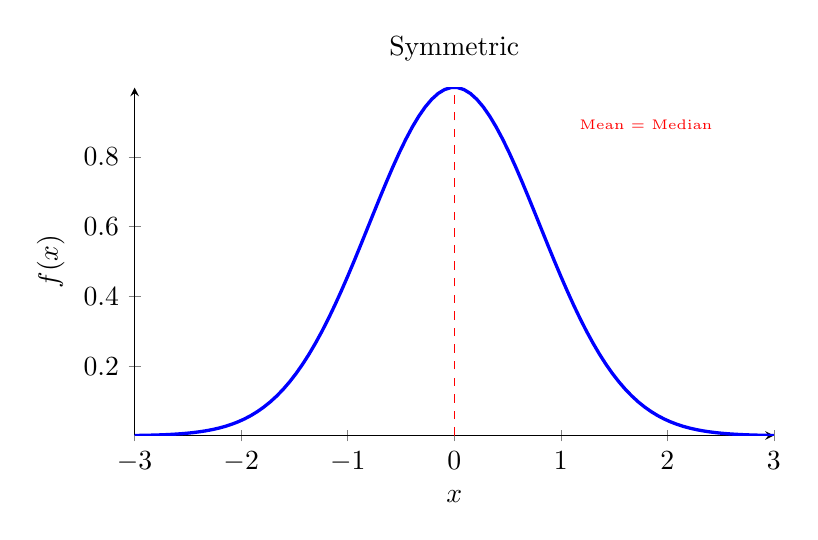
\begin{tikzpicture}
          \begin{axis}[
              domain=-3:3,
              samples=100,
              xlabel={$x$},
              ylabel={$f(x)$},
              axis lines=left,
              width=0.8\textwidth,
              height=6cm,
              title={Symmetric}
            ]
            % Plot a symmetric bell-shaped curve (scaled normal)
            \addplot[very thick, blue] {exp(-0.5*(x/0.8)^2)};
            % Mark the common mean and median
            \draw[dashed, red] (axis cs:0,0) -- (axis cs:0,{exp(-0.5*(0/0.8)^2)});
            \node[red, above] at (axis cs:1.8,0.85) {\tiny Mean = Median};
          \end{axis}
        \end{tikzpicture}
    \end{column}

    % Right column (larger) with dot plot
    \hspace{-2em}
    \begin{column}{0.3\textwidth}
    \footnotesize
     A symmetric distribution is a distribution in which the shape on the left and right sides of the center are mirror images of each other, meaning that the frequencies change at the same rate and direction as one moves away from the center in both directions.
    \end{column}
\end{columns}

\end{frame}



%%%%%%%%%%%%%%%%%%%%%%%%%%%%%%%%%%%%%%%%%%%%%%%%%%%%%%%%%%%%%%%%%%%%%%%%%%%
\section{Histograms}
\transitionslide{Histograms}

% Slide 1: Introduction to Histograms
\begin{frame}{Introduction to Histograms}
    \textbf{What is a Histogram?}
    \begin{itemize}
        \item A histogram is a graphical representation of the distribution of numerical data.
        \item It uses bins (or intervals) to group data points and shows the frequency of data points in each bin.
        \item The height of each bar represents the count or frequency of data within that bin.
    \end{itemize}
\end{frame}

% Slide 2: Step 1 - Understanding Absolute Frequency
\begin{frame}{Step 1: Understanding Absolute Frequency}
    \textbf{Absolute Frequency:}
    \begin{itemize}
        \item The absolute frequency of an interval is the number of data points that fall within that interval.
        \item It's simply a count of occurrences of data points in each interval.
    \end{itemize}

    \vspace{0.5cm}
    \textbf{Example:}
    \begin{itemize}
        \item Consider the data: \{3, 5, 7, 9, 11, 5, 7, 9, 3, 5\}
        \item The absolute frequency of the interval [3, 6] is 5 (as four data points fall in this interval: 3, 3, 5, 5, 5).
    \end{itemize}
\end{frame}

% Slide 3: Step 2 - Choosing Bins (Intervals)
\begin{frame}{Step 2: Choosing Bins (Intervals)}
    \textbf{What are Bins?}
    \begin{itemize}
        \item Bins (or intervals) divide the entire range of values into equal-sized chunks.
        \item Each bin contains a specific range of values, and data points are placed into the bin they fall within.
    \end{itemize}

    \vspace{0.5cm}

    \textbf{General Definition:}
    \begin{itemize}
        \item \emph{First} bin: \([ \text{min}, \text{min} + \text{bin\_size} )\)
        \item Bin \(k\): \([ \text{min} + (k-1)\cdot\text{bin\_size} , \text{min} +  (k) \cdot \text{bin\_size}  )\)
        \item \emph{Last} bin: \([ \text{max}-\text{bin\_size}, \text{max}   ]\)
        \begin{itemize}
            \item It’s normal to close the last bin on the right to capture the maximum.
        \end{itemize}
    \end{itemize}
\end{frame}


% Slide 4: Step 3 - Assigning Data to Bins
\begin{frame}{Step 3: Assigning Data to Bins}
    \textbf{Assigning Data to Bins:}
    \begin{itemize}
        \item Once bins are defined, we assign each data point to the appropriate bin.
        \item This process results in an absolute frequency count for each bin.
    \end{itemize}

    \vspace{0.5cm}
    \textbf{Example:}
    \begin{itemize}
        \item Suppose a discrete variable that goes from 1 to 15.
        \item Suppose we have 3 bins: [1, 6), [6, 11), [11, 15].
        \item If the data is \{3, 7, 9, 12, 3, 5\}, then:
        \begin{itemize}
            \item Bin [1, 6): 3 data points \{3, 3, 5\}
            \item Bin [6, 11): 2 data points \{7, 9\}
            \item Bin [11, 15]: 1 data point \{12\}
        \end{itemize}
    \end{itemize}
\end{frame}

% Slide 5: Step 4 - Constructing the Histogram
\begin{frame}{Step 4: Constructing the Histogram}
    \textbf{Constructing the Histogram:}
    \begin{itemize}
        \item Now that we have the counts (absolute frequencies) for each bin, we can construct the histogram.
        \item The x-axis represents the bin intervals, and the y-axis represents the count of data points in each bin.
        \item Draw a bar for each bin where the height corresponds to the count (absolute frequency).
    \end{itemize}
\end{frame}

% Slide 6: Example of Histogram Construction - Data Table
\begin{frame}{Example: Data Table}
    \textbf{Step-by-Step Example:}
    \vspace{0.5cm}
    Consider the following data set:

    \begin{center}
        \begin{tabular}{cccccccccc}
            3 & 5 & 7 & 9 & 11 & 3 & 4 & 6 & 8 & 10 \\
            12 & 15 & 1 & 2 & 14 & 5 & 7 & 9 & 11 & 13 \\
        \end{tabular}
    \end{center}

    \vspace{0.5cm}
    We will construct a histogram with 5 bins.
\end{frame}

% Slide 7: Example of Histogram Construction - Correct Binning and Plotting
\begin{frame}{Example: Histogram with 5 Bins }
    \textbf{Step-by-Step Example:}
    \begin{itemize}
        \item Range of data: 1 to 15
        \item Bin size = \( \frac{15 - 1}{5} = 2.8 \) (rounded to 3)
        \item Bins:
        \begin{itemize}
            \item \([1, 4)\): 4 data points \{1, 2, 3, 3\}
            \item \([4, 7)\): 4 data points \{4, 5, 5, 6\}
            \item \([7, 10)\): 5 data points \{7, 7, 8, 9, 9\}
            \item \([10, 13)\): 4 data points \{10, 11, 11, 12\}
            \item \([13, 15]\): 3 data points \{13, 14, 15\}
        \end{itemize}
    \end{itemize}


\end{frame}

% Slide 7: Example of Histogram Construction - Binning and Plotting (Corrected)
\begin{frame}{Example: Histogram with 5 Bins}

    \begin{center}
        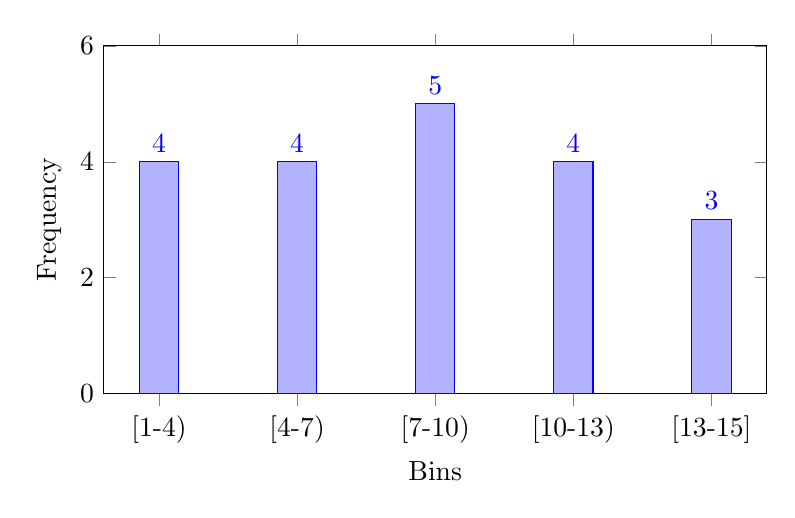
\begin{tikzpicture}
            \begin{axis}[
                ybar,
                symbolic x coords={[1-4), [4-7), [7-10), [10-13), [13-15]},
                xtick=data,
                ymin=0,
                ymax=6,
                bar width=0.5cm,
                xlabel={Bins},
                ylabel={Frequency},
                width=10cm, height=6cm,
                nodes near coords            ]
            % Updated frequencies and correct bin intervals
            \addplot coordinates {([1-4),4)  ([4-7),4) ([7-10),5) ([10-13),4) ([13-15],3)};
            \end{axis}
        \end{tikzpicture}
    \end{center}
\end{frame}

%%%%%%%%%%%%%%%%%%%%%%%%%%%%%%%%%%%%%%%%%%%%%%%%%%%%%%%%%%%%%%%%%%%%%%%%%%%
\section{Bar Plots}
\transitionslide{Bar Plots}

% Slide 1: Introduction to Bar Plots
\begin{frame}{When Do We Use Bar Plots?}
    \textbf{Bar Plots:}
    \begin{itemize}
        \item Bar plots are used to display the frequency or proportion of categorical data.
        \item They are especially useful for comparing different categories.
        \item Each bar represents a category, and the height of the bar represents the value (frequency, proportion, etc.).
    \end{itemize}

    \vspace{0.5cm}
    \textbf{Use Cases:}
    \begin{itemize}
        \item Visualizing survey responses.
        \item Comparing the frequency of different groups (e.g., gender, age groups).
    \end{itemize}
\end{frame}



% Slide 3: What is a Frequency Distribution?
\begin{frame}{What is a Frequency Distribution?}
    \textbf{Frequency Distribution:}
    \begin{itemize}
        \item A frequency distribution is a table that shows the frequency (or count) of each value or category.
        \item It can be visualized using a bar plot where each category corresponds to a bar.
    \end{itemize}

    \vspace{0.5cm}
    \textbf{Example:}
    \begin{center}
        \begin{tabular}{lc}
            \toprule
            \textbf{Category} & \textbf{Frequency} \\
            \midrule
            A & 10 \\
            B & 15 \\
            C & 5 \\
            \bottomrule
        \end{tabular}
    \end{center}

\end{frame}

% Slide 2: Basic Bar Plot Structure
\begin{frame}{Basic Bar Plot Structure}
    \begin{itemize}
        \item The x-axis represents categories (e.g., different groups).
        \item The y-axis represents the frequency, proportion, or value corresponding to each category.
        \item Bars can be vertical or horizontal.
    \end{itemize}

\pgfplotstableread[row sep=\\,col sep=&]{
    categ & freq \\
    A   &   10  \\
    B   &   15  \\
    C   &   5 \\
    }\mydata

\begin{center}
\begin{tikzpicture}
    \begin{axis}[
            ybar,
            bar width=.5cm,
            width=\textwidth,
            height=.5\textwidth,
            symbolic x coords={A,B,C},
            xtick=data,
            nodes near coords,
            nodes near coords align={vertical},
            ymin=0,ymax=20,
            ylabel={Frequency},
            width=0.6\textwidth,
            nodes near coords,
            enlarge x limits=0.4, % Reduce the extra space around bars
            axis on top, % Ensure axis is on top
            tick align=inside, % Align ticks inside to avoid extra spacing
        ]
        \addplot table[x=categ,y=freq]{\mydata};
    \end{axis}
\end{tikzpicture}
\end{center}

\end{frame}


% Slide 4: What is Cross-Tabulation?
\begin{frame}{What is Cross-Tabulation?}
    \textbf{Cross-Tabulation (Crosstab):}
    \begin{itemize}
        \item Cross-tabulation is a method used to analyze the relationship between two categorical variables.
        \item It creates a matrix (or table) that shows the frequency distribution of the variables across their categories.
    \end{itemize}

    \vspace{0.5cm}
    \textbf{Example:}
    \begin{center}
        \begin{tabular}{lcc}
            \toprule
            & \textbf{Group 1} & \textbf{Group 2} \\
            \midrule
            Category A & 5 & 8 \\
            Category B & 10 & 12 \\
            \bottomrule
        \end{tabular}
    \end{center}
\end{frame}

% Slide 5: Bar Plots for Cross-Tabulation
\begin{frame}{Using Bar Plots for Cross-Tabulation}
    \textbf{Bar Plots for Two Variables:}
    \begin{itemize}
        \item Bar plots can also represent cross-tabulation by plotting grouped bars.
        \item Each group (e.g., Group 1, Group 2) has its own bar for each category.
    \end{itemize}

    \textbf{Example:}
    \begin{center}
        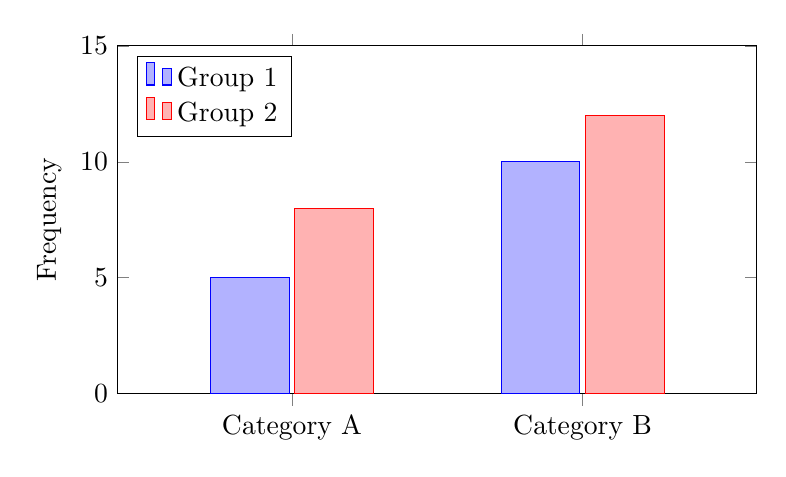
\begin{tikzpicture}
            \begin{axis}[
                ybar,
                symbolic x coords={Category A, Category B},
                xtick=data,
                ymin=0,
                ymax=15,
                bar width=1cm,
                width=10cm, height=6cm,
                ylabel={Frequency},
                legend pos=north west,
                width=0.8\textwidth,
                enlarge x limits=0.6 % Reduce the extra space around bars
            ]
            \addplot coordinates {(Category A,5) (Category B,10)};
            \addplot coordinates {(Category A,8) (Category B,12)};
            \legend{Group 1, Group 2}
            \end{axis}
        \end{tikzpicture}
    \end{center}

\end{frame}

% Slide 5: Bar Plots for Cross-Tabulation
\begin{frame}{Using Bar Plots for Cross-Tabulation}
    \textbf{Stacked Bar Plots for Two Variables:}
    \begin{itemize}
        \item Bar plots can also be \emph{stacked} within each category.
        \item We often do this when we represent percentages in the $y$-axis.
    \end{itemize}

    \textbf{Example:}
    \begin{center}
        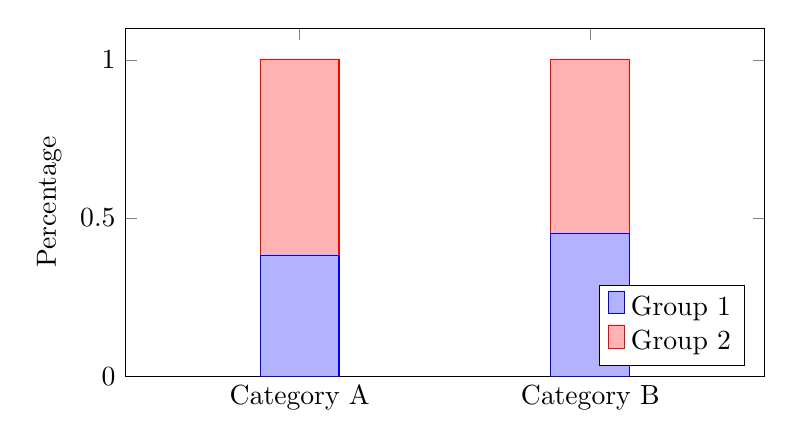
\begin{tikzpicture}
            \begin{axis}[
                ybar stacked,
                symbolic x coords={Category A, Category B},
                xtick=data,
                ymin=0,
                ymax=1.1,
                bar width=1cm,
                width=10cm, height=6cm,
                ylabel={Percentage},
                legend pos=south east,
                width=0.8\textwidth,
                enlarge x limits=0.6 % Reduce the extra space around bars
            ]
            \addplot coordinates {(Category A,.38) (Category B,0.45)};
            \addplot coordinates {(Category A,.62) (Category B,0.55)};
            \legend{Group 1, Group 2}
            \end{axis}
        \end{tikzpicture}
    \end{center}

\end{frame}

%%%%%%%%%%%%%%%%%%%%%%%%%%%%%%%%%%%%%%%%%%%%%%%%%%%%%%%%%%%%%%%%%%%%%%%%%%%
\section{Box Plots}
\transitionslide{Box Plots}

% Slide 1: Introduction to Box Plots
\begin{frame}{Introduction to Box Plots}
    \begin{itemize}
        \item A box plot (or box-and-whisker plot) displays the distribution of quantitative data in a way that facilitates comparisons between variables or across levels of a categorical variable.
        \item The box shows the quartiles of the dataset while the whiskers extend to show the rest of the distribution, except for points that are determined to be “outliers” using a method that is a function of the inter-quartile range.
        \item Box plots give a clear summary of data distribution and variability and are particularly useful for highlighting outliers and for comparing distributions across groups.
    \end{itemize}
\end{frame}

% Slide 2: Constructing a Box Plot
\begin{frame}{Constructing a Box Plot}
    \textbf{Steps to Construct a Box Plot:}
    \begin{enumerate}
        \item Calculate the first (Q1) and third quartiles (Q3).
        \item Find the interquartile range (IQR = Q3 - Q1).
        \item Determine the “whiskers” which are typically set at 1.5 * IQR above Q3 and below Q1. Data points outside this range are considered outliers.
        \item The median (Q2) is marked by a line inside the box. If a distribution is skewed, then the median will not be in the middle of the box, and instead off to the side.
    \end{enumerate}

\end{frame}

\begin{frame}{Structure of a Box Plot}
\centering
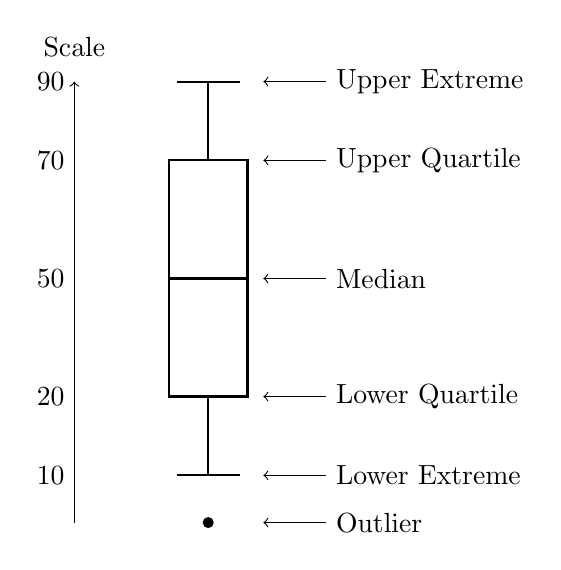
\begin{tikzpicture}

% Boxplot
\draw[thick] (3,1.5) rectangle (4,4.5);  % Draw the box from lower to upper quartile
\draw[thick] (3.5,0.5) -- (3.5,1.5);    % Lower whisker
\draw[thick] (3.5,4.5) -- (3.5,5.5);    % Upper whisker
\draw[thick] (3,3) -- (4,3);            % Median line
\draw[thick] (3.1,0.5) -- (3.9,0.5);      % Lower extreme horizontal line
\draw[thick] (3.1,5.5) -- (3.9,5.5);      % Upper extreme horizontal line
\fill (3.5,-.1) circle (2pt);          % Outlier point

% Labels
\draw[<-] (4.2,5.5) -- (5,5.5) node[right] {Upper Extreme};
\draw[<-] (4.2,4.5) -- (5,4.5) node[right] {Upper Quartile};
\draw[<-] (4.2,3) -- (5,3) node[right] {Median};
\draw[<-] (4.2,1.5) -- (5,1.5) node[right] {Lower Quartile};
\draw[<-] (4.2,-0.10) -- (5,-0.10) node[right] {Outlier};
\draw[<-] (4.2,0.5) -- (5,0.5) node[right] {Lower Extreme};

% Y-axis scale
\foreach \y/\label in {0.5/10, 1.5/20, 3/50, 4.5/70, 5.5/90}
    \draw (1.8,\y) node[left] {\label};

\draw[<-] (1.8,5.5) -- (1.8,-0.10);
\draw (1.8,5.7) node[above] {Scale};

\end{tikzpicture}
\end{frame}

\begin{frame}{Example: Box Plot with Multiple Categories}
\centering
    \begin{tikzpicture}
	\pgfplotstableread[col sep=comma]{data.csv}\csvdata
	% Boxplot groups columns, but we want rows
	\pgfplotstabletranspose\datatransposed{\csvdata}
	\begin{axis}[
		boxplot/draw direction = y,
		x axis line style = {opacity=0},
		axis x line* = bottom,
		axis y line = left,
		enlarge y limits,
		ymajorgrids,
		xtick = {1, 2, 3, 4},
		xticklabel style = {align=center, font=\small, rotate=60},
		xticklabels = {Apples, Oranges, Bananas, Melons},
		xtick style = {draw=none}, % Hide tick line
		ylabel = {Juiciness},
		ytick = {10, 20, 30, 40},
        ymax = 42,
        ymin = 6
	]
		\foreach \n in {1,...,4} {
			\addplot+[boxplot, fill, draw=black] table[y index=\n] {\datatransposed};
		}
	\end{axis}
\end{tikzpicture}

\end{frame}

%%%%%%%%%%%%%%%%%%%%%%%%%%%%%%%%%%%%%%%%%%%%%%%%%%%%%%%%%%%%%%%%%%%%%%%%%%%
\section{Dot Charts}
\transitionslide{Dot Charts}

% Slide 1: Introduction to Dot Charts
\begin{frame}{Introduction to Dot Charts}
    \textbf{What is a Dot Chart?}
    \begin{itemize}
        \item A dot chart is a statistical chart consisting of data points plotted on a simple scale.
        \item It is used to compare frequency, count, or any measure across different categories.
        \item Similar to bar charts but dots are used instead of bars, making it less cluttered.
    \end{itemize}
    \textbf{Why Use Dot Charts?}
    \begin{itemize}
        \item \textbf{Clarity:} Provides a clear and precise representation of data points.
        \item \textbf{Comparison:} Facilitates easy comparison of multiple groups.
        \item \textbf{Space-efficient:} More effective in space usage than bar graphs.
    \end{itemize}
\end{frame}


% Slide 3: Comparing Means Across Groups Using Dot Charts
\begin{frame}{Comparing Means Across Groups Using Dot Charts}
    \textbf{How to Use Dot Charts for Comparing Means}
    \begin{itemize}
        \item Dot charts are excellent for displaying the mean (or any central tendency) of different groups.
        \item Each dot represents the mean of a group, aligned along a single axis.
        \item The position of each dot on the scale directly reflects the value of the mean, making comparisons intuitive.
    \end{itemize}

    \textbf{Example:}
    \begin{center}
        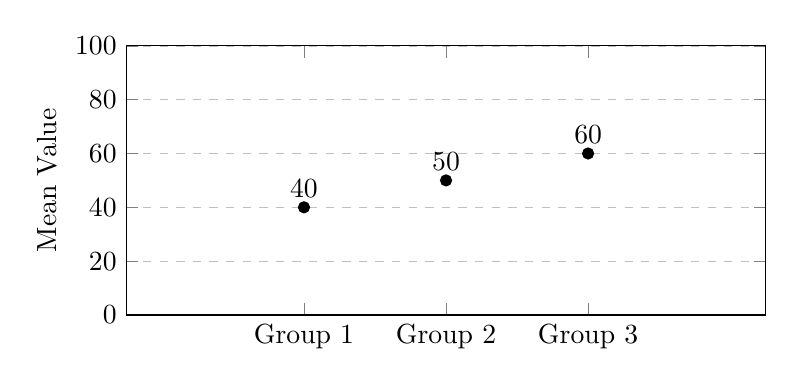
\begin{tikzpicture}
            \begin{axis}[
                only marks,
                ylabel={Mean Value},
                width=0.8\textwidth,
                height=6cm,
                xtick=data,
                xticklabels={Group 1, Group 2, Group 3},
                xmin=0.5, xmax=3.5,
                ymin=0, ymax=100,
                enlarge x limits=0.25,
                height=5cm,
                ymajorgrids=true, % Enable major grids for y-axis only
                grid style={line width=.1pt, draw=gray!10}, % Light gray color for grid lines
                major grid style={line width=.2pt,draw=gray!50, dashed}
            ]
            \addplot[mark=*, nodes near coords] coordinates {(1, 40) (2, 50) (3, 60)};
            \end{axis}
        \end{tikzpicture}
    \end{center}
\end{frame}

%%%%%%%%%%%%%%%%%%%%%%%%%%%%%%%%%%%%%%%%%%%%%%%%%%%%%%%%%%%%%%%%%%%%%%%%%%%
\section{Scatter Plot}
\transitionslide{Scatter Plot}

\begin{frame}{Introduction to Scatter Plots}
    \textbf{What is a Scatter Plot?}
    \begin{itemize}
        \item A scatter plot is a type of data visualization that shows the relationship between two numerical variables.
        \item Each point on the plot represents a pair of values: one on the x-axis and one on the y-axis.
        \item Scatter plots are useful for identifying correlations, trends, and outliers in data.
    \end{itemize}

    \textbf{Applications of Scatter Plots}
    \begin{itemize}
        \item Visualizing correlations between variables.
        \item Spotting clusters and patterns.
        \item Detecting outliers and anomalies.
    \end{itemize}
\end{frame}

\begin{frame}{How to Create a Scatter Plot}
    \textbf{Steps to Create a Scatter Plot:}
    \begin{itemize}
        \item \textbf{Step 1:} Gather your data points. You need two variables, one for the x-axis and one for the y-axis.
        \item \textbf{Step 2:} Plot each pair of values on a coordinate system.
        \item \textbf{Step 3:} Optionally, add labels, grid lines, and color coding to enhance interpretation.
    \end{itemize}

    \textbf{Example:}
    \begin{itemize}
        \item Dataset: (1,2), (2,3), (3,6), (4,7), (5,10)
        \item The scatter plot will show these points in a linear relationship.
    \end{itemize}
\end{frame}

\begin{frame}{Scatter Plot Example (Basic)}
    \textbf{Example of a Scatter Plot:}

    \begin{center}
        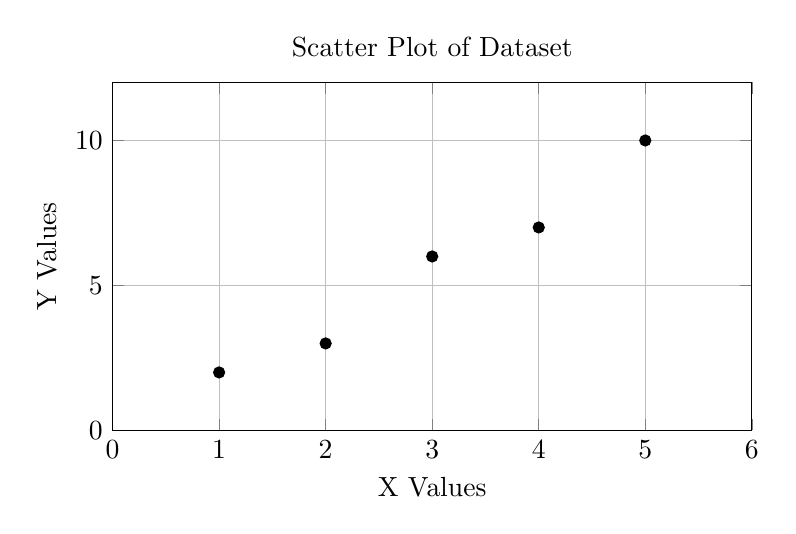
\begin{tikzpicture}
            \begin{axis}[
                title={Scatter Plot of Dataset},
                xlabel={X Values},
                ylabel={Y Values},
                width=0.8\textwidth,
                height=6cm,
                grid=major,
                ymin=0, ymax=12,
                xmin=0, xmax=6,
                scatter/classes={
                    a={mark=*,black},b={mark=*,black},c={mark=*,black}
                }
            ]
            \addplot[scatter,only marks,scatter src=explicit symbolic]
            coordinates {
                (1,2) [a] (2,3) [b] (3,6) [a] (4,7) [b] (5,10) [c]
            };
            \end{axis}
        \end{tikzpicture}
    \end{center}
\end{frame}

\begin{frame}{Scatter Plot Example with Two Classes }

Imagine our dataset has two classes (Class A and Class B).

    \begin{center}
        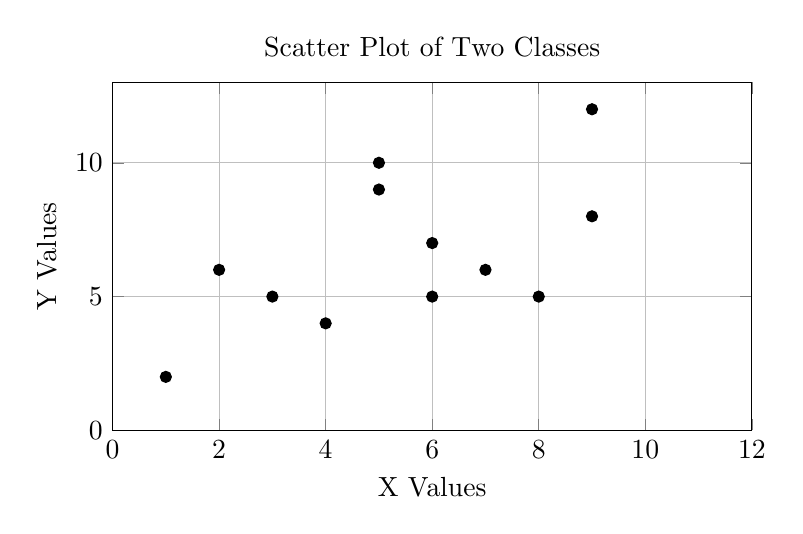
\begin{tikzpicture}
            \begin{axis}[
                title={Scatter Plot of Two Classes},
                xlabel={X Values},
                ylabel={Y Values},
                width=0.8\textwidth,
                height=6cm,
                grid=major,
                ymin=0, ymax=13,
                xmin=0, xmax=12,
                scatter/classes={
                    a={mark=*,black},b={mark=*,black}
                }
            ]
            % Adding more points for each class
            \addplot[scatter,only marks,scatter src=explicit symbolic]
            coordinates {
                (1,2) [a] (2,6) [b] (3,5) [a] (4,4) [b] (5,10) [a] (6,5) [a]
                (7,6) [b] (8,5) [b] (9,8) [b] (6,7) [a] (5,9) [b] (9,12) [a]
            };
            \end{axis}
        \end{tikzpicture}
    \end{center}

\end{frame}



\begin{frame}{Scatter Plot Example with Two Classes }

We have two different classes (Class A and Class B), each represented by different colors:
        \begin{itemize}
            \item Blue: Class A
            \item Red: Class B
        \end{itemize}

    \begin{center}
        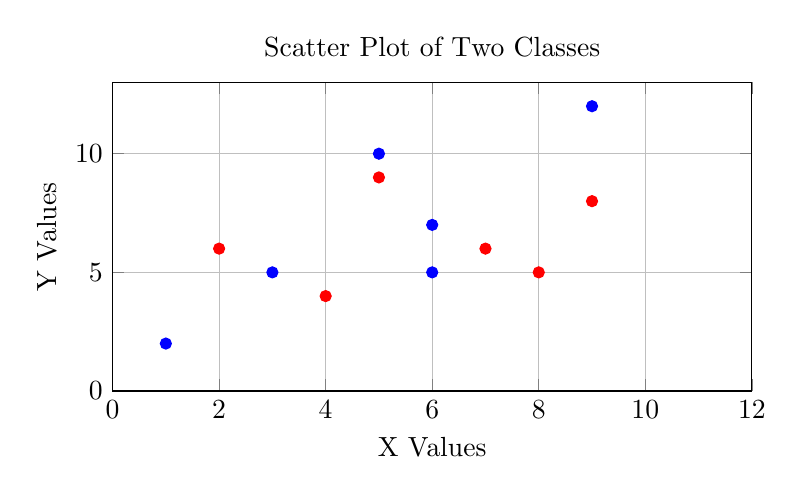
\begin{tikzpicture}
            \begin{axis}[
                title={Scatter Plot of Two Classes},
                xlabel={X Values},
                ylabel={Y Values},
                width=0.8\textwidth,
                height=5.5cm,
                grid=major,
                ymin=0, ymax=13,
                xmin=0, xmax=12,
                scatter/classes={
                    a={mark=*,blue},b={mark=*,red}
                }
            ]
            % Adding more points for each class
            \addplot[scatter,only marks,scatter src=explicit symbolic]
            coordinates {
                (1,2) [a] (2,6) [b] (3,5) [a] (4,4) [b] (5,10) [a] (6,5) [a]
                (7,6) [b] (8,5) [b] (9,8) [b] (6,7) [a] (5,9) [b] (9,12) [a]
            };
            \end{axis}
        \end{tikzpicture}
    \end{center}

\end{frame}


\begin{frame}{Side-by-Side Comparison}
    \begin{minipage}[t]{0.48\textwidth}
        \begin{center}
        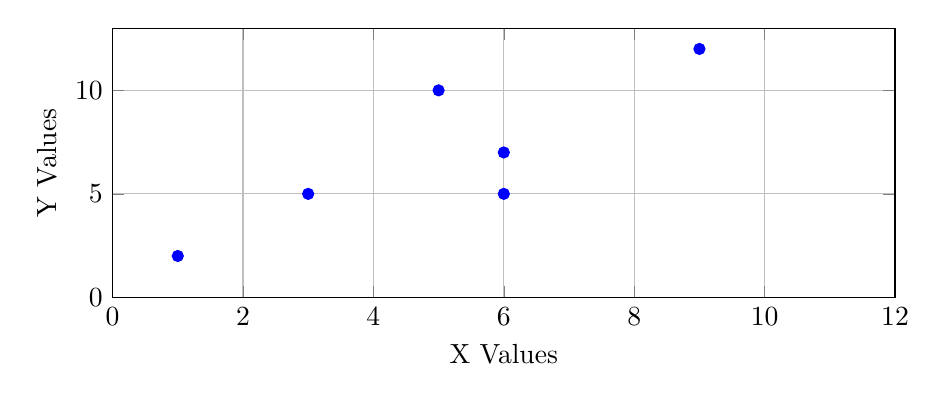
\begin{tikzpicture}
            \begin{axis}[
                xlabel={X Values},
                ylabel={Y Values},
                width=0.95\textwidth,
                height=5cm,
                grid=major,
                ymin=0, ymax=13,
                xmin=0, xmax=12,
                scatter/classes={
                    a={mark=*,blue},b={mark=*,red!0,fill opacity = 0.0001, draw opacity = 0.0001}
                }
            ]
            % Adding more points for each class
            \addplot[scatter,only marks,scatter src=explicit symbolic]
            coordinates {
                (1,2) [a] (2,6) [b] (3,5) [a] (4,4) [b] (5,10) [a] (6,5) [a]
                (7,6) [b] (8,5) [b] (9,8) [b] (6,7) [a] (5,9) [b] (9,12) [a]
            };
            \end{axis}
        \end{tikzpicture}
    \end{center}
    \end{minipage}
    \hfill
    \begin{minipage}[t]{0.48\textwidth}
\begin{center}
        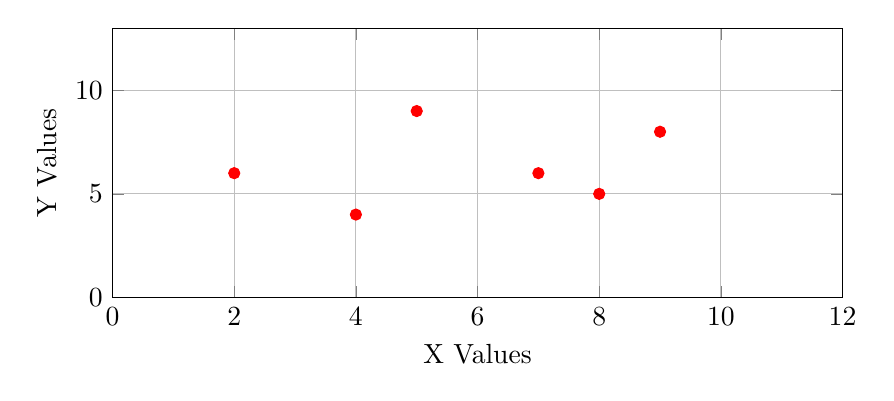
\begin{tikzpicture}
            \begin{axis}[
                xlabel={X Values},
                ylabel={Y Values},
                width=0.895\textwidth,
                height=5cm,
                grid=major,
                ymin=0, ymax=13,
                xmin=0, xmax=12,
                scatter/classes={
                    a={mark=*,red!0,fill opacity = 0.0001, draw opacity = 0.0001},b={mark=*,red}
                }
            ]
            % Adding more points for each class
            \addplot[scatter,only marks,scatter src=explicit symbolic]
            coordinates {
                (1,2) [a] (2,6) [b] (3,5) [a] (4,4) [b] (5,10) [a] (6,5) [a]
                (7,6) [b] (8,5) [b] (9,8) [b] (6,7) [a] (5,9) [b] (9,12) [a]
            };
            \end{axis}
        \end{tikzpicture}
    \end{center}
    \end{minipage}
\end{frame}

%%%%%%%%%%%%%%%%%%%%%%%%%%%%%%%%%%%%%%%%%%%%%%%%%%%%%%%%%%%%%%%%%%%%%%%%%%%
\section{Summary and Takeaways}
\transitionslide{Summary and Takeaways}

\begin{frame}{Summary: Distributions and Plots}
    \textbf{Key Takeaways:}
    \begin{itemize}
        \item \textbf{Shape of Distribution:} Understand skewness (right, left) and mode (unimodal, bimodal, multimodal).
        \item \textbf{Histogram:} Useful for visualizing the distribution of intervals or bins of data.
        \item \textbf{Bar Plot:} Best for categorical data comparisons.
        \item \textbf{Box Plot:} Ideal for displaying the distribution's quartiles and identifying outliers.
        \item \textbf{Dot Chart:} Great for comparing multiple categories without the clutter of bars.
        \item \textbf{Scatter Plot:} Essential for identifying relationships and trends between two variables.
    \end{itemize}
\end{frame}

\end{document}
